\documentclass[11pt,a4paper]{amsart}

\usepackage[margin=2.8cm]{geometry}
\usepackage{microtype}
\usepackage{amsmath,amssymb,amsthm}
\usepackage{booktabs}
\usepackage{tikz}
\usepackage{pgfplots}
\usepackage{pgfplotstable}
\pgfplotsset{compat=1.18}
\usepackage[labelfont=bf]{caption}
\usepackage{subcaption}
\usepackage[hidelinks]{hyperref}

\newtheorem{theorem}{Theorem}[section]
\newtheorem{lemma}[theorem]{Lemma}
\newtheorem{proposition}[theorem]{Proposition}
\newtheorem{corollary}[theorem]{Corollary}
\theoremstyle{definition}
\newtheorem{definition}[theorem]{Definition}
\theoremstyle{remark}
\newtheorem{remark}[theorem]{Remark}

\newcommand{\R}{\mathbb{R}}
\newcommand{\Q}{Q}
\newcommand{\Prob}{\mathbb{P}}
\newcommand{\eps}{\varepsilon}
\newcommand{\repo}{\url{https://github.com/diegor117/hex-brouwer-percolation}}

% Styles shared by the generated figures (paper/figures/*.tex).
\tikzset{
  stoneblack/.style={fill=black!85, draw=black!45, line width=0.3pt},
  stonewhite/.style={fill=white, draw=black!45, line width=0.3pt},
  frameblack/.style={fill=black!50, draw=black!45, line width=0.3pt},
  framewhite/.style={fill=black!8, draw=black!45, line width=0.3pt},
  fence/.style={draw=red!75!black, line width=0.7pt},
  walk/.style={draw=red!80!black, line width=1.5pt, line cap=round, line join=round},
  endpoint/.style={fill=red!80!black},
  chainmark/.style={fill=red!80!black},
  label/.style={font=\small},
  gblack/.style={fill=black!85},
  gwhite/.style={fill=white},
  gblank/.style={fill=black!35},
  gframe/.style={draw=black, line width=0.5pt},
  fixed/.style={draw=red!80!black, line width=1.2pt},
}

\title[The Hex theorem, Brouwer's theorem and a crossing probability]{The Hex theorem, Brouwer's fixed-point theorem,\\ and a crossing probability equal to one half}

\author{Diego Rapini}
\author{Luigi Lanni}
\author{Massimiliano Iorio}

\date{October 2026}


\begin{document}

\begin{abstract}
We give a self-contained account of three classical facts about the board game Hex. First, a completely filled Hex board contains a winning chain for exactly one of the two players; we present Gale's path-following proof that at least one player has a chain, and refer to Huneke for the proof that at most one does. Second, following Gale, we deduce the Brouwer fixed-point theorem for the unit square from the Hex theorem. Third, if every cell of an $n \times n$ board is coloured black independently with probability $p$, the probability $\theta_n(p)$ of a black top-to-bottom chain satisfies $\theta_n(p) + \theta_n(1-p) = 1$; in particular $\theta_n(1/2) = 1/2$ for every $n$. We check these statements numerically with the code that accompanies the paper, by exhaustive enumeration for $n \le 5$ and by Monte Carlo sampling for larger boards. None of the results is new.
\end{abstract}

\maketitle

\section{Introduction}

Hex was invented by the Danish designer Piet Hein, who published it under the name \emph{Polygon} in the newspaper \emph{Politiken} in December 1942, and independently by John Nash at Princeton around 1948. Martin Gardner described it in his Scientific American column of July 1957 \cite{gardner}. A detailed history is given by Hayward and Toft \cite{hayward-toft}.

Two players, Black and White, alternately place stones of their colour on the empty cells of a board of hexagonal cells shaped like a rhombus (Figure~\ref{fig:walk}). Black tries to connect the top and bottom edges of the board with a chain of adjacent black stones, and White tries to connect the left and right edges with a chain of white stones. Stones are never moved or removed. Hein required that a game of Hex cannot end in a draw. Nash showed by a strategy-stealing argument that the first player has a winning strategy on every board; the argument does not say what the strategy is.

The statement that a draw is impossible is a theorem about colourings of the board (Theorem~\ref{thm:hex}). In 1979 Gale \cite{gale} gave a short proof of it by following a path between the two colours, and showed that the Hex theorem and the Brouwer fixed-point theorem in dimension two can each be derived from the other by elementary means.

This paper is organised as follows. Section~\ref{sec:hex} states the Hex theorem and gives Gale's proof that at least one player has a winning chain. Section~\ref{sec:brouwer} derives the Brouwer fixed-point theorem for the square from it. Section~\ref{sec:perc} treats random colourings and proves that the probability of a black crossing on a square board is $1/2$ when $p = 1/2$. Section~\ref{sec:numerics} reports the numerical checks. The code, the test suite and interactive versions of the figures are available at \repo.

\section{The Hex theorem}\label{sec:hex}

\begin{definition}
The \emph{$n \times n$ Hex board} $H_n$ is the set of cells $(r,c)$ with $r, c \in \{0, \dots, n-1\}$, where $r$ is the row (counted from the top) and $c$ is the column (counted from the left). Each cell is a regular hexagon, and the hexagons are arranged so that two cells share an edge if and only if their difference is one of
\[
  \pm(0,1), \qquad \pm(1,0), \qquad \pm(1,-1).
\]
Such cells are called \emph{adjacent}. A \emph{colouring} of $H_n$ assigns to every cell one of the colours black and white. A \emph{black crossing} is a sequence of black cells, each adjacent to the next, starting in row $0$ and ending in row $n-1$. A \emph{white crossing} is a sequence of white cells, each adjacent to the next, starting in column $0$ and ending in column $n-1$.
\end{definition}

\begin{theorem}[Hex theorem]\label{thm:hex}
For every colouring of $H_n$, exactly one of the following holds: there is a black crossing, or there is a white crossing.
\end{theorem}

Because stones are never removed, a game that continues until the board is full ends in a colouring of $H_n$, and Theorem~\ref{thm:hex} shows that one of the players has completed a chain by then. We prove the two halves of the theorem separately.

\subsection{At least one crossing}

We follow Gale \cite{gale}. Fix a colouring of $H_n$ and add a frame around the board: two rows of black cells $(-1,c)$ and $(n,c)$, and two columns of white cells $(r,-1)$ and $(r,n)$, for $0 \le r, c \le n-1$. The frame colours agree with the edges that each player owns. Let $F_n$ be the set of cells of the board and the frame, and let $R \subset \R^2$ be the union of their hexagons.

A \emph{fence} is an edge of the hexagonal tiling that is shared by two cells of $F_n$ of different colours. Let $G$ be the graph whose vertices are the vertices of the tiling that lie in $R$ and whose edges are the fences. Figure~\ref{fig:walk-a} shows the fences for one colouring.

\begin{lemma}\label{lem:degrees}
\begin{enumerate}
  \item[(a)] Every vertex of $G$ in the interior of $R$ has degree $0$ or $2$.
  \item[(b)] Exactly four vertices of $G$ have degree $1$. They lie on the boundary of $R$, one near each corner of the board. All other boundary vertices have degree $0$.
\end{enumerate}
\end{lemma}

\begin{proof}
(a) Exactly three hexagons of the tiling meet at each vertex. If they all have the same colour, no fence ends at the vertex. Otherwise the colours split two against one, and the fences ending at the vertex are the two edges of the minority hexagon that meet there (Figure~\ref{fig:vertex}). This is the step that uses the hexagonal shape of the cells: on a square grid four cells meet at a vertex, and the fences can cross there.

(b) A vertex on the boundary of $R$ lies on one or two cells of $F_n$. If it lies on one, it has degree $0$. If it lies on two, these two cells share an edge ending at the vertex, and the vertex has degree $1$ when the two cells have different colours and degree $0$ otherwise. The cells that meet the boundary of $R$ are the frame cells and the two board cells $(0,n-1)$ and $(n-1,0)$ at the obtuse corners. Going once around the boundary, starting at the top-left corner, they appear in the order: the top frame row (black), the cell $(0,n-1)$, the right frame column (white), the bottom frame row (black), the cell $(n-1,0)$, the left frame column (white). Whatever the colours of $(0,n-1)$ and $(n-1,0)$, the colour changes exactly four times along this cycle, once near each corner. Each change gives one vertex of degree $1$.
\end{proof}

\begin{figure}[t]
  \centering
  \begin{subfigure}[b]{0.49\textwidth}
    \centering
    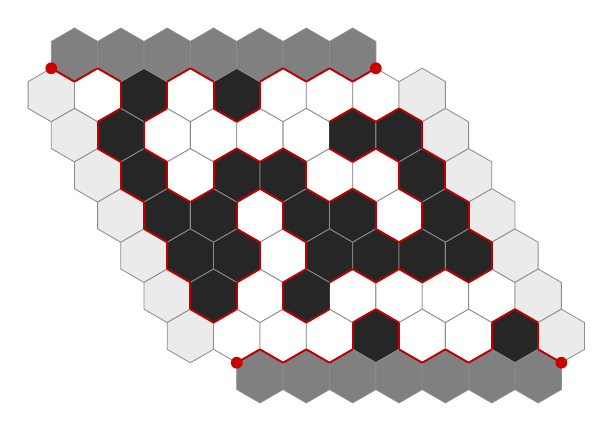
\begin{tikzpicture}[x=0.34cm,y=0.34cm]
      \filldraw[stonewhite] (0.866,-0.500)--(0,-1.000)--(-0.866,-0.500)--(-0.866,0.500)--(0,1.000)--(0.866,0.500)--cycle;
\filldraw[stoneblack] (2.598,-0.500)--(1.732,-1.000)--(0.866,-0.500)--(0.866,0.500)--(1.732,1.000)--(2.598,0.500)--cycle;
\filldraw[stonewhite] (4.330,-0.500)--(3.464,-1.000)--(2.598,-0.500)--(2.598,0.500)--(3.464,1.000)--(4.330,0.500)--cycle;
\filldraw[stoneblack] (6.062,-0.500)--(5.196,-1.000)--(4.330,-0.500)--(4.330,0.500)--(5.196,1.000)--(6.062,0.500)--cycle;
\filldraw[stonewhite] (7.794,-0.500)--(6.928,-1.000)--(6.062,-0.500)--(6.062,0.500)--(6.928,1.000)--(7.794,0.500)--cycle;
\filldraw[stonewhite] (9.526,-0.500)--(8.660,-1.000)--(7.794,-0.500)--(7.794,0.500)--(8.660,1.000)--(9.526,0.500)--cycle;
\filldraw[stonewhite] (11.258,-0.500)--(10.392,-1.000)--(9.526,-0.500)--(9.526,0.500)--(10.392,1.000)--(11.258,0.500)--cycle;
\filldraw[stoneblack] (1.732,-2.000)--(0.866,-2.500)--(0,-2.000)--(0,-1.000)--(0.866,-0.500)--(1.732,-1.000)--cycle;
\filldraw[stonewhite] (3.464,-2.000)--(2.598,-2.500)--(1.732,-2.000)--(1.732,-1.000)--(2.598,-0.500)--(3.464,-1.000)--cycle;
\filldraw[stonewhite] (5.196,-2.000)--(4.330,-2.500)--(3.464,-2.000)--(3.464,-1.000)--(4.330,-0.500)--(5.196,-1.000)--cycle;
\filldraw[stonewhite] (6.928,-2.000)--(6.062,-2.500)--(5.196,-2.000)--(5.196,-1.000)--(6.062,-0.500)--(6.928,-1.000)--cycle;
\filldraw[stonewhite] (8.660,-2.000)--(7.794,-2.500)--(6.928,-2.000)--(6.928,-1.000)--(7.794,-0.500)--(8.660,-1.000)--cycle;
\filldraw[stoneblack] (10.392,-2.000)--(9.526,-2.500)--(8.660,-2.000)--(8.660,-1.000)--(9.526,-0.500)--(10.392,-1.000)--cycle;
\filldraw[stoneblack] (12.124,-2.000)--(11.258,-2.500)--(10.392,-2.000)--(10.392,-1.000)--(11.258,-0.500)--(12.124,-1.000)--cycle;
\filldraw[stoneblack] (2.598,-3.500)--(1.732,-4.000)--(0.866,-3.500)--(0.866,-2.500)--(1.732,-2.000)--(2.598,-2.500)--cycle;
\filldraw[stonewhite] (4.330,-3.500)--(3.464,-4.000)--(2.598,-3.500)--(2.598,-2.500)--(3.464,-2.000)--(4.330,-2.500)--cycle;
\filldraw[stoneblack] (6.062,-3.500)--(5.196,-4.000)--(4.330,-3.500)--(4.330,-2.500)--(5.196,-2.000)--(6.062,-2.500)--cycle;
\filldraw[stoneblack] (7.794,-3.500)--(6.928,-4.000)--(6.062,-3.500)--(6.062,-2.500)--(6.928,-2.000)--(7.794,-2.500)--cycle;
\filldraw[stonewhite] (9.526,-3.500)--(8.660,-4.000)--(7.794,-3.500)--(7.794,-2.500)--(8.660,-2.000)--(9.526,-2.500)--cycle;
\filldraw[stonewhite] (11.258,-3.500)--(10.392,-4.000)--(9.526,-3.500)--(9.526,-2.500)--(10.392,-2.000)--(11.258,-2.500)--cycle;
\filldraw[stoneblack] (12.990,-3.500)--(12.124,-4.000)--(11.258,-3.500)--(11.258,-2.500)--(12.124,-2.000)--(12.990,-2.500)--cycle;
\filldraw[stoneblack] (3.464,-5.000)--(2.598,-5.500)--(1.732,-5.000)--(1.732,-4.000)--(2.598,-3.500)--(3.464,-4.000)--cycle;
\filldraw[stoneblack] (5.196,-5.000)--(4.330,-5.500)--(3.464,-5.000)--(3.464,-4.000)--(4.330,-3.500)--(5.196,-4.000)--cycle;
\filldraw[stonewhite] (6.928,-5.000)--(6.062,-5.500)--(5.196,-5.000)--(5.196,-4.000)--(6.062,-3.500)--(6.928,-4.000)--cycle;
\filldraw[stoneblack] (8.660,-5.000)--(7.794,-5.500)--(6.928,-5.000)--(6.928,-4.000)--(7.794,-3.500)--(8.660,-4.000)--cycle;
\filldraw[stoneblack] (10.392,-5.000)--(9.526,-5.500)--(8.660,-5.000)--(8.660,-4.000)--(9.526,-3.500)--(10.392,-4.000)--cycle;
\filldraw[stonewhite] (12.124,-5.000)--(11.258,-5.500)--(10.392,-5.000)--(10.392,-4.000)--(11.258,-3.500)--(12.124,-4.000)--cycle;
\filldraw[stoneblack] (13.856,-5.000)--(12.990,-5.500)--(12.124,-5.000)--(12.124,-4.000)--(12.990,-3.500)--(13.856,-4.000)--cycle;
\filldraw[stoneblack] (4.330,-6.500)--(3.464,-7.000)--(2.598,-6.500)--(2.598,-5.500)--(3.464,-5.000)--(4.330,-5.500)--cycle;
\filldraw[stoneblack] (6.062,-6.500)--(5.196,-7.000)--(4.330,-6.500)--(4.330,-5.500)--(5.196,-5.000)--(6.062,-5.500)--cycle;
\filldraw[stonewhite] (7.794,-6.500)--(6.928,-7.000)--(6.062,-6.500)--(6.062,-5.500)--(6.928,-5.000)--(7.794,-5.500)--cycle;
\filldraw[stoneblack] (9.526,-6.500)--(8.660,-7.000)--(7.794,-6.500)--(7.794,-5.500)--(8.660,-5.000)--(9.526,-5.500)--cycle;
\filldraw[stoneblack] (11.258,-6.500)--(10.392,-7.000)--(9.526,-6.500)--(9.526,-5.500)--(10.392,-5.000)--(11.258,-5.500)--cycle;
\filldraw[stoneblack] (12.990,-6.500)--(12.124,-7.000)--(11.258,-6.500)--(11.258,-5.500)--(12.124,-5.000)--(12.990,-5.500)--cycle;
\filldraw[stoneblack] (14.722,-6.500)--(13.856,-7.000)--(12.990,-6.500)--(12.990,-5.500)--(13.856,-5.000)--(14.722,-5.500)--cycle;
\filldraw[stoneblack] (5.196,-8.000)--(4.330,-8.500)--(3.464,-8.000)--(3.464,-7.000)--(4.330,-6.500)--(5.196,-7.000)--cycle;
\filldraw[stonewhite] (6.928,-8.000)--(6.062,-8.500)--(5.196,-8.000)--(5.196,-7.000)--(6.062,-6.500)--(6.928,-7.000)--cycle;
\filldraw[stoneblack] (8.660,-8.000)--(7.794,-8.500)--(6.928,-8.000)--(6.928,-7.000)--(7.794,-6.500)--(8.660,-7.000)--cycle;
\filldraw[stonewhite] (10.392,-8.000)--(9.526,-8.500)--(8.660,-8.000)--(8.660,-7.000)--(9.526,-6.500)--(10.392,-7.000)--cycle;
\filldraw[stonewhite] (12.124,-8.000)--(11.258,-8.500)--(10.392,-8.000)--(10.392,-7.000)--(11.258,-6.500)--(12.124,-7.000)--cycle;
\filldraw[stonewhite] (13.856,-8.000)--(12.990,-8.500)--(12.124,-8.000)--(12.124,-7.000)--(12.990,-6.500)--(13.856,-7.000)--cycle;
\filldraw[stonewhite] (15.588,-8.000)--(14.722,-8.500)--(13.856,-8.000)--(13.856,-7.000)--(14.722,-6.500)--(15.588,-7.000)--cycle;
\filldraw[stonewhite] (6.062,-9.500)--(5.196,-10.000)--(4.330,-9.500)--(4.330,-8.500)--(5.196,-8.000)--(6.062,-8.500)--cycle;
\filldraw[stonewhite] (7.794,-9.500)--(6.928,-10.000)--(6.062,-9.500)--(6.062,-8.500)--(6.928,-8.000)--(7.794,-8.500)--cycle;
\filldraw[stonewhite] (9.526,-9.500)--(8.660,-10.000)--(7.794,-9.500)--(7.794,-8.500)--(8.660,-8.000)--(9.526,-8.500)--cycle;
\filldraw[stoneblack] (11.258,-9.500)--(10.392,-10.000)--(9.526,-9.500)--(9.526,-8.500)--(10.392,-8.000)--(11.258,-8.500)--cycle;
\filldraw[stonewhite] (12.990,-9.500)--(12.124,-10.000)--(11.258,-9.500)--(11.258,-8.500)--(12.124,-8.000)--(12.990,-8.500)--cycle;
\filldraw[stonewhite] (14.722,-9.500)--(13.856,-10.000)--(12.990,-9.500)--(12.990,-8.500)--(13.856,-8.000)--(14.722,-8.500)--cycle;
\filldraw[stoneblack] (16.454,-9.500)--(15.588,-10.000)--(14.722,-9.500)--(14.722,-8.500)--(15.588,-8.000)--(16.454,-8.500)--cycle;
\filldraw[frameblack] (0,1.000)--(-0.866,0.500)--(-1.732,1.000)--(-1.732,2.000)--(-0.866,2.500)--(0,2.000)--cycle;
\filldraw[frameblack] (6.928,-11.000)--(6.062,-11.500)--(5.196,-11.000)--(5.196,-10.000)--(6.062,-9.500)--(6.928,-10.000)--cycle;
\filldraw[frameblack] (1.732,1.000)--(0.866,0.500)--(0,1.000)--(0,2.000)--(0.866,2.500)--(1.732,2.000)--cycle;
\filldraw[frameblack] (8.660,-11.000)--(7.794,-11.500)--(6.928,-11.000)--(6.928,-10.000)--(7.794,-9.500)--(8.660,-10.000)--cycle;
\filldraw[frameblack] (3.464,1.000)--(2.598,0.500)--(1.732,1.000)--(1.732,2.000)--(2.598,2.500)--(3.464,2.000)--cycle;
\filldraw[frameblack] (10.392,-11.000)--(9.526,-11.500)--(8.660,-11.000)--(8.660,-10.000)--(9.526,-9.500)--(10.392,-10.000)--cycle;
\filldraw[frameblack] (5.196,1.000)--(4.330,0.500)--(3.464,1.000)--(3.464,2.000)--(4.330,2.500)--(5.196,2.000)--cycle;
\filldraw[frameblack] (12.124,-11.000)--(11.258,-11.500)--(10.392,-11.000)--(10.392,-10.000)--(11.258,-9.500)--(12.124,-10.000)--cycle;
\filldraw[frameblack] (6.928,1.000)--(6.062,0.500)--(5.196,1.000)--(5.196,2.000)--(6.062,2.500)--(6.928,2.000)--cycle;
\filldraw[frameblack] (13.856,-11.000)--(12.990,-11.500)--(12.124,-11.000)--(12.124,-10.000)--(12.990,-9.500)--(13.856,-10.000)--cycle;
\filldraw[frameblack] (8.660,1.000)--(7.794,0.500)--(6.928,1.000)--(6.928,2.000)--(7.794,2.500)--(8.660,2.000)--cycle;
\filldraw[frameblack] (15.588,-11.000)--(14.722,-11.500)--(13.856,-11.000)--(13.856,-10.000)--(14.722,-9.500)--(15.588,-10.000)--cycle;
\filldraw[frameblack] (10.392,1.000)--(9.526,0.500)--(8.660,1.000)--(8.660,2.000)--(9.526,2.500)--(10.392,2.000)--cycle;
\filldraw[frameblack] (17.321,-11.000)--(16.454,-11.500)--(15.588,-11.000)--(15.588,-10.000)--(16.454,-9.500)--(17.321,-10.000)--cycle;
\filldraw[framewhite] (-0.866,-0.500)--(-1.732,-1.000)--(-2.598,-0.500)--(-2.598,0.500)--(-1.732,1.000)--(-0.866,0.500)--cycle;
\filldraw[framewhite] (12.990,-0.500)--(12.124,-1.000)--(11.258,-0.500)--(11.258,0.500)--(12.124,1.000)--(12.990,0.500)--cycle;
\filldraw[framewhite] (0,-2.000)--(-0.866,-2.500)--(-1.732,-2.000)--(-1.732,-1.000)--(-0.866,-0.500)--(0,-1.000)--cycle;
\filldraw[framewhite] (13.856,-2.000)--(12.990,-2.500)--(12.124,-2.000)--(12.124,-1.000)--(12.990,-0.500)--(13.856,-1.000)--cycle;
\filldraw[framewhite] (0.866,-3.500)--(0,-4.000)--(-0.866,-3.500)--(-0.866,-2.500)--(0,-2.000)--(0.866,-2.500)--cycle;
\filldraw[framewhite] (14.722,-3.500)--(13.856,-4.000)--(12.990,-3.500)--(12.990,-2.500)--(13.856,-2.000)--(14.722,-2.500)--cycle;
\filldraw[framewhite] (1.732,-5.000)--(0.866,-5.500)--(0,-5.000)--(0,-4.000)--(0.866,-3.500)--(1.732,-4.000)--cycle;
\filldraw[framewhite] (15.588,-5.000)--(14.722,-5.500)--(13.856,-5.000)--(13.856,-4.000)--(14.722,-3.500)--(15.588,-4.000)--cycle;
\filldraw[framewhite] (2.598,-6.500)--(1.732,-7.000)--(0.866,-6.500)--(0.866,-5.500)--(1.732,-5.000)--(2.598,-5.500)--cycle;
\filldraw[framewhite] (16.454,-6.500)--(15.588,-7.000)--(14.722,-6.500)--(14.722,-5.500)--(15.588,-5.000)--(16.454,-5.500)--cycle;
\filldraw[framewhite] (3.464,-8.000)--(2.598,-8.500)--(1.732,-8.000)--(1.732,-7.000)--(2.598,-6.500)--(3.464,-7.000)--cycle;
\filldraw[framewhite] (17.321,-8.000)--(16.454,-8.500)--(15.588,-8.000)--(15.588,-7.000)--(16.454,-6.500)--(17.321,-7.000)--cycle;
\filldraw[framewhite] (4.330,-9.500)--(3.464,-10.000)--(2.598,-9.500)--(2.598,-8.500)--(3.464,-8.000)--(4.330,-8.500)--cycle;
\filldraw[framewhite] (18.187,-9.500)--(17.321,-10.000)--(16.454,-9.500)--(16.454,-8.500)--(17.321,-8.000)--(18.187,-8.500)--cycle;
\draw[fence] (0.866,-0.500)--(0,-1.000);
\draw[fence] (0.866,-0.500)--(0.866,0.500);
\draw[fence] (0,-1.000)--(0,-2.000);
\draw[fence] (-0.866,0.500)--(0,1.000);
\draw[fence] (-0.866,0.500)--(-1.732,1.000);
\draw[fence] (0,1.000)--(0.866,0.500);
\draw[fence] (2.598,-0.500)--(1.732,-1.000);
\draw[fence] (2.598,-0.500)--(2.598,0.500);
\draw[fence] (1.732,-1.000)--(1.732,-2.000);
\draw[fence] (2.598,0.500)--(3.464,1.000);
\draw[fence] (3.464,1.000)--(4.330,0.500);
\draw[fence] (4.330,0.500)--(4.330,-0.500);
\draw[fence] (4.330,-0.500)--(5.196,-1.000);
\draw[fence] (6.062,-0.500)--(5.196,-1.000);
\draw[fence] (6.062,-0.500)--(6.062,0.500);
\draw[fence] (6.062,0.500)--(6.928,1.000);
\draw[fence] (6.928,1.000)--(7.794,0.500);
\draw[fence] (7.794,0.500)--(8.660,1.000);
\draw[fence] (9.526,-0.500)--(8.660,-1.000);
\draw[fence] (9.526,-0.500)--(10.392,-1.000);
\draw[fence] (8.660,-1.000)--(8.660,-2.000);
\draw[fence] (8.660,1.000)--(9.526,0.500);
\draw[fence] (9.526,0.500)--(10.392,1.000);
\draw[fence] (11.258,-0.500)--(10.392,-1.000);
\draw[fence] (11.258,-0.500)--(12.124,-1.000);
\draw[fence] (0.866,-2.500)--(0,-2.000);
\draw[fence] (0.866,-2.500)--(0.866,-3.500);
\draw[fence] (1.732,-2.000)--(2.598,-2.500);
\draw[fence] (2.598,-2.500)--(2.598,-3.500);
\draw[fence] (5.196,-2.000)--(4.330,-2.500);
\draw[fence] (5.196,-2.000)--(6.062,-2.500);
\draw[fence] (4.330,-2.500)--(4.330,-3.500);
\draw[fence] (6.928,-2.000)--(6.062,-2.500);
\draw[fence] (6.928,-2.000)--(7.794,-2.500);
\draw[fence] (7.794,-2.500)--(7.794,-3.500);
\draw[fence] (8.660,-2.000)--(9.526,-2.500);
\draw[fence] (10.392,-2.000)--(9.526,-2.500);
\draw[fence] (10.392,-2.000)--(11.258,-2.500);
\draw[fence] (11.258,-2.500)--(11.258,-3.500);
\draw[fence] (12.124,-1.000)--(12.124,-2.000);
\draw[fence] (12.124,-2.000)--(12.990,-2.500);
\draw[fence] (1.732,-4.000)--(0.866,-3.500);
\draw[fence] (1.732,-4.000)--(1.732,-5.000);
\draw[fence] (2.598,-3.500)--(3.464,-4.000);
\draw[fence] (4.330,-3.500)--(3.464,-4.000);
\draw[fence] (6.062,-3.500)--(5.196,-4.000);
\draw[fence] (6.062,-3.500)--(6.928,-4.000);
\draw[fence] (5.196,-4.000)--(5.196,-5.000);
\draw[fence] (6.928,-4.000)--(6.928,-5.000);
\draw[fence] (7.794,-3.500)--(8.660,-4.000);
\draw[fence] (9.526,-3.500)--(8.660,-4.000);
\draw[fence] (9.526,-3.500)--(10.392,-4.000);
\draw[fence] (10.392,-4.000)--(10.392,-5.000);
\draw[fence] (11.258,-3.500)--(12.124,-4.000);
\draw[fence] (12.124,-4.000)--(12.124,-5.000);
\draw[fence] (12.990,-2.500)--(12.990,-3.500);
\draw[fence] (12.990,-3.500)--(13.856,-4.000);
\draw[fence] (2.598,-5.500)--(1.732,-5.000);
\draw[fence] (2.598,-5.500)--(2.598,-6.500);
\draw[fence] (5.196,-5.000)--(6.062,-5.500);
\draw[fence] (6.062,-5.500)--(6.062,-6.500);
\draw[fence] (6.928,-5.000)--(7.794,-5.500);
\draw[fence] (7.794,-5.500)--(7.794,-6.500);
\draw[fence] (10.392,-5.000)--(11.258,-5.500);
\draw[fence] (12.124,-5.000)--(11.258,-5.500);
\draw[fence] (13.856,-4.000)--(13.856,-5.000);
\draw[fence] (13.856,-5.000)--(14.722,-5.500);
\draw[fence] (3.464,-7.000)--(2.598,-6.500);
\draw[fence] (3.464,-7.000)--(3.464,-8.000);
\draw[fence] (6.062,-6.500)--(5.196,-7.000);
\draw[fence] (5.196,-7.000)--(5.196,-8.000);
\draw[fence] (7.794,-6.500)--(6.928,-7.000);
\draw[fence] (6.928,-7.000)--(6.928,-8.000);
\draw[fence] (9.526,-6.500)--(8.660,-7.000);
\draw[fence] (9.526,-6.500)--(10.392,-7.000);
\draw[fence] (8.660,-7.000)--(8.660,-8.000);
\draw[fence] (11.258,-6.500)--(10.392,-7.000);
\draw[fence] (11.258,-6.500)--(12.124,-7.000);
\draw[fence] (12.990,-6.500)--(12.124,-7.000);
\draw[fence] (12.990,-6.500)--(13.856,-7.000);
\draw[fence] (14.722,-6.500)--(13.856,-7.000);
\draw[fence] (14.722,-6.500)--(14.722,-5.500);
\draw[fence] (5.196,-8.000)--(4.330,-8.500);
\draw[fence] (4.330,-8.500)--(3.464,-8.000);
\draw[fence] (6.928,-8.000)--(7.794,-8.500);
\draw[fence] (8.660,-8.000)--(7.794,-8.500);
\draw[fence] (10.392,-8.000)--(9.526,-8.500);
\draw[fence] (10.392,-8.000)--(11.258,-8.500);
\draw[fence] (9.526,-8.500)--(9.526,-9.500);
\draw[fence] (11.258,-8.500)--(11.258,-9.500);
\draw[fence] (15.588,-8.000)--(14.722,-8.500);
\draw[fence] (15.588,-8.000)--(16.454,-8.500);
\draw[fence] (14.722,-8.500)--(14.722,-9.500);
\draw[fence] (6.062,-9.500)--(5.196,-10.000);
\draw[fence] (6.062,-9.500)--(6.928,-10.000);
\draw[fence] (7.794,-9.500)--(6.928,-10.000);
\draw[fence] (7.794,-9.500)--(8.660,-10.000);
\draw[fence] (9.526,-9.500)--(8.660,-10.000);
\draw[fence] (11.258,-9.500)--(12.124,-10.000);
\draw[fence] (12.990,-9.500)--(12.124,-10.000);
\draw[fence] (12.990,-9.500)--(13.856,-10.000);
\draw[fence] (14.722,-9.500)--(13.856,-10.000);
\draw[fence] (16.454,-8.500)--(16.454,-9.500);
\draw[fence] (16.454,-9.500)--(17.321,-10.000);
\fill[endpoint] (10.392,1.000) circle (0.22);
\fill[endpoint] (5.196,-10.000) circle (0.22);
\fill[endpoint] (-1.732,1.000) circle (0.22);
\fill[endpoint] (17.321,-10.000) circle (0.22);

    \end{tikzpicture}
    \caption{Fences and the four vertices of degree 1.}\label{fig:walk-a}
  \end{subfigure}\hfill
  \begin{subfigure}[b]{0.49\textwidth}
    \centering
    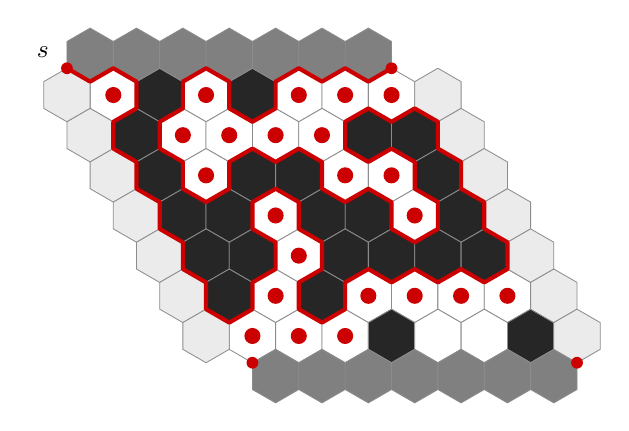
\begin{tikzpicture}[x=0.34cm,y=0.34cm]
      \filldraw[stonewhite] (0.866,-0.500)--(0,-1.000)--(-0.866,-0.500)--(-0.866,0.500)--(0,1.000)--(0.866,0.500)--cycle;
\filldraw[stoneblack] (2.598,-0.500)--(1.732,-1.000)--(0.866,-0.500)--(0.866,0.500)--(1.732,1.000)--(2.598,0.500)--cycle;
\filldraw[stonewhite] (4.330,-0.500)--(3.464,-1.000)--(2.598,-0.500)--(2.598,0.500)--(3.464,1.000)--(4.330,0.500)--cycle;
\filldraw[stoneblack] (6.062,-0.500)--(5.196,-1.000)--(4.330,-0.500)--(4.330,0.500)--(5.196,1.000)--(6.062,0.500)--cycle;
\filldraw[stonewhite] (7.794,-0.500)--(6.928,-1.000)--(6.062,-0.500)--(6.062,0.500)--(6.928,1.000)--(7.794,0.500)--cycle;
\filldraw[stonewhite] (9.526,-0.500)--(8.660,-1.000)--(7.794,-0.500)--(7.794,0.500)--(8.660,1.000)--(9.526,0.500)--cycle;
\filldraw[stonewhite] (11.258,-0.500)--(10.392,-1.000)--(9.526,-0.500)--(9.526,0.500)--(10.392,1.000)--(11.258,0.500)--cycle;
\filldraw[stoneblack] (1.732,-2.000)--(0.866,-2.500)--(0,-2.000)--(0,-1.000)--(0.866,-0.500)--(1.732,-1.000)--cycle;
\filldraw[stonewhite] (3.464,-2.000)--(2.598,-2.500)--(1.732,-2.000)--(1.732,-1.000)--(2.598,-0.500)--(3.464,-1.000)--cycle;
\filldraw[stonewhite] (5.196,-2.000)--(4.330,-2.500)--(3.464,-2.000)--(3.464,-1.000)--(4.330,-0.500)--(5.196,-1.000)--cycle;
\filldraw[stonewhite] (6.928,-2.000)--(6.062,-2.500)--(5.196,-2.000)--(5.196,-1.000)--(6.062,-0.500)--(6.928,-1.000)--cycle;
\filldraw[stonewhite] (8.660,-2.000)--(7.794,-2.500)--(6.928,-2.000)--(6.928,-1.000)--(7.794,-0.500)--(8.660,-1.000)--cycle;
\filldraw[stoneblack] (10.392,-2.000)--(9.526,-2.500)--(8.660,-2.000)--(8.660,-1.000)--(9.526,-0.500)--(10.392,-1.000)--cycle;
\filldraw[stoneblack] (12.124,-2.000)--(11.258,-2.500)--(10.392,-2.000)--(10.392,-1.000)--(11.258,-0.500)--(12.124,-1.000)--cycle;
\filldraw[stoneblack] (2.598,-3.500)--(1.732,-4.000)--(0.866,-3.500)--(0.866,-2.500)--(1.732,-2.000)--(2.598,-2.500)--cycle;
\filldraw[stonewhite] (4.330,-3.500)--(3.464,-4.000)--(2.598,-3.500)--(2.598,-2.500)--(3.464,-2.000)--(4.330,-2.500)--cycle;
\filldraw[stoneblack] (6.062,-3.500)--(5.196,-4.000)--(4.330,-3.500)--(4.330,-2.500)--(5.196,-2.000)--(6.062,-2.500)--cycle;
\filldraw[stoneblack] (7.794,-3.500)--(6.928,-4.000)--(6.062,-3.500)--(6.062,-2.500)--(6.928,-2.000)--(7.794,-2.500)--cycle;
\filldraw[stonewhite] (9.526,-3.500)--(8.660,-4.000)--(7.794,-3.500)--(7.794,-2.500)--(8.660,-2.000)--(9.526,-2.500)--cycle;
\filldraw[stonewhite] (11.258,-3.500)--(10.392,-4.000)--(9.526,-3.500)--(9.526,-2.500)--(10.392,-2.000)--(11.258,-2.500)--cycle;
\filldraw[stoneblack] (12.990,-3.500)--(12.124,-4.000)--(11.258,-3.500)--(11.258,-2.500)--(12.124,-2.000)--(12.990,-2.500)--cycle;
\filldraw[stoneblack] (3.464,-5.000)--(2.598,-5.500)--(1.732,-5.000)--(1.732,-4.000)--(2.598,-3.500)--(3.464,-4.000)--cycle;
\filldraw[stoneblack] (5.196,-5.000)--(4.330,-5.500)--(3.464,-5.000)--(3.464,-4.000)--(4.330,-3.500)--(5.196,-4.000)--cycle;
\filldraw[stonewhite] (6.928,-5.000)--(6.062,-5.500)--(5.196,-5.000)--(5.196,-4.000)--(6.062,-3.500)--(6.928,-4.000)--cycle;
\filldraw[stoneblack] (8.660,-5.000)--(7.794,-5.500)--(6.928,-5.000)--(6.928,-4.000)--(7.794,-3.500)--(8.660,-4.000)--cycle;
\filldraw[stoneblack] (10.392,-5.000)--(9.526,-5.500)--(8.660,-5.000)--(8.660,-4.000)--(9.526,-3.500)--(10.392,-4.000)--cycle;
\filldraw[stonewhite] (12.124,-5.000)--(11.258,-5.500)--(10.392,-5.000)--(10.392,-4.000)--(11.258,-3.500)--(12.124,-4.000)--cycle;
\filldraw[stoneblack] (13.856,-5.000)--(12.990,-5.500)--(12.124,-5.000)--(12.124,-4.000)--(12.990,-3.500)--(13.856,-4.000)--cycle;
\filldraw[stoneblack] (4.330,-6.500)--(3.464,-7.000)--(2.598,-6.500)--(2.598,-5.500)--(3.464,-5.000)--(4.330,-5.500)--cycle;
\filldraw[stoneblack] (6.062,-6.500)--(5.196,-7.000)--(4.330,-6.500)--(4.330,-5.500)--(5.196,-5.000)--(6.062,-5.500)--cycle;
\filldraw[stonewhite] (7.794,-6.500)--(6.928,-7.000)--(6.062,-6.500)--(6.062,-5.500)--(6.928,-5.000)--(7.794,-5.500)--cycle;
\filldraw[stoneblack] (9.526,-6.500)--(8.660,-7.000)--(7.794,-6.500)--(7.794,-5.500)--(8.660,-5.000)--(9.526,-5.500)--cycle;
\filldraw[stoneblack] (11.258,-6.500)--(10.392,-7.000)--(9.526,-6.500)--(9.526,-5.500)--(10.392,-5.000)--(11.258,-5.500)--cycle;
\filldraw[stoneblack] (12.990,-6.500)--(12.124,-7.000)--(11.258,-6.500)--(11.258,-5.500)--(12.124,-5.000)--(12.990,-5.500)--cycle;
\filldraw[stoneblack] (14.722,-6.500)--(13.856,-7.000)--(12.990,-6.500)--(12.990,-5.500)--(13.856,-5.000)--(14.722,-5.500)--cycle;
\filldraw[stoneblack] (5.196,-8.000)--(4.330,-8.500)--(3.464,-8.000)--(3.464,-7.000)--(4.330,-6.500)--(5.196,-7.000)--cycle;
\filldraw[stonewhite] (6.928,-8.000)--(6.062,-8.500)--(5.196,-8.000)--(5.196,-7.000)--(6.062,-6.500)--(6.928,-7.000)--cycle;
\filldraw[stoneblack] (8.660,-8.000)--(7.794,-8.500)--(6.928,-8.000)--(6.928,-7.000)--(7.794,-6.500)--(8.660,-7.000)--cycle;
\filldraw[stonewhite] (10.392,-8.000)--(9.526,-8.500)--(8.660,-8.000)--(8.660,-7.000)--(9.526,-6.500)--(10.392,-7.000)--cycle;
\filldraw[stonewhite] (12.124,-8.000)--(11.258,-8.500)--(10.392,-8.000)--(10.392,-7.000)--(11.258,-6.500)--(12.124,-7.000)--cycle;
\filldraw[stonewhite] (13.856,-8.000)--(12.990,-8.500)--(12.124,-8.000)--(12.124,-7.000)--(12.990,-6.500)--(13.856,-7.000)--cycle;
\filldraw[stonewhite] (15.588,-8.000)--(14.722,-8.500)--(13.856,-8.000)--(13.856,-7.000)--(14.722,-6.500)--(15.588,-7.000)--cycle;
\filldraw[stonewhite] (6.062,-9.500)--(5.196,-10.000)--(4.330,-9.500)--(4.330,-8.500)--(5.196,-8.000)--(6.062,-8.500)--cycle;
\filldraw[stonewhite] (7.794,-9.500)--(6.928,-10.000)--(6.062,-9.500)--(6.062,-8.500)--(6.928,-8.000)--(7.794,-8.500)--cycle;
\filldraw[stonewhite] (9.526,-9.500)--(8.660,-10.000)--(7.794,-9.500)--(7.794,-8.500)--(8.660,-8.000)--(9.526,-8.500)--cycle;
\filldraw[stoneblack] (11.258,-9.500)--(10.392,-10.000)--(9.526,-9.500)--(9.526,-8.500)--(10.392,-8.000)--(11.258,-8.500)--cycle;
\filldraw[stonewhite] (12.990,-9.500)--(12.124,-10.000)--(11.258,-9.500)--(11.258,-8.500)--(12.124,-8.000)--(12.990,-8.500)--cycle;
\filldraw[stonewhite] (14.722,-9.500)--(13.856,-10.000)--(12.990,-9.500)--(12.990,-8.500)--(13.856,-8.000)--(14.722,-8.500)--cycle;
\filldraw[stoneblack] (16.454,-9.500)--(15.588,-10.000)--(14.722,-9.500)--(14.722,-8.500)--(15.588,-8.000)--(16.454,-8.500)--cycle;
\filldraw[frameblack] (0,1.000)--(-0.866,0.500)--(-1.732,1.000)--(-1.732,2.000)--(-0.866,2.500)--(0,2.000)--cycle;
\filldraw[frameblack] (6.928,-11.000)--(6.062,-11.500)--(5.196,-11.000)--(5.196,-10.000)--(6.062,-9.500)--(6.928,-10.000)--cycle;
\filldraw[frameblack] (1.732,1.000)--(0.866,0.500)--(0,1.000)--(0,2.000)--(0.866,2.500)--(1.732,2.000)--cycle;
\filldraw[frameblack] (8.660,-11.000)--(7.794,-11.500)--(6.928,-11.000)--(6.928,-10.000)--(7.794,-9.500)--(8.660,-10.000)--cycle;
\filldraw[frameblack] (3.464,1.000)--(2.598,0.500)--(1.732,1.000)--(1.732,2.000)--(2.598,2.500)--(3.464,2.000)--cycle;
\filldraw[frameblack] (10.392,-11.000)--(9.526,-11.500)--(8.660,-11.000)--(8.660,-10.000)--(9.526,-9.500)--(10.392,-10.000)--cycle;
\filldraw[frameblack] (5.196,1.000)--(4.330,0.500)--(3.464,1.000)--(3.464,2.000)--(4.330,2.500)--(5.196,2.000)--cycle;
\filldraw[frameblack] (12.124,-11.000)--(11.258,-11.500)--(10.392,-11.000)--(10.392,-10.000)--(11.258,-9.500)--(12.124,-10.000)--cycle;
\filldraw[frameblack] (6.928,1.000)--(6.062,0.500)--(5.196,1.000)--(5.196,2.000)--(6.062,2.500)--(6.928,2.000)--cycle;
\filldraw[frameblack] (13.856,-11.000)--(12.990,-11.500)--(12.124,-11.000)--(12.124,-10.000)--(12.990,-9.500)--(13.856,-10.000)--cycle;
\filldraw[frameblack] (8.660,1.000)--(7.794,0.500)--(6.928,1.000)--(6.928,2.000)--(7.794,2.500)--(8.660,2.000)--cycle;
\filldraw[frameblack] (15.588,-11.000)--(14.722,-11.500)--(13.856,-11.000)--(13.856,-10.000)--(14.722,-9.500)--(15.588,-10.000)--cycle;
\filldraw[frameblack] (10.392,1.000)--(9.526,0.500)--(8.660,1.000)--(8.660,2.000)--(9.526,2.500)--(10.392,2.000)--cycle;
\filldraw[frameblack] (17.321,-11.000)--(16.454,-11.500)--(15.588,-11.000)--(15.588,-10.000)--(16.454,-9.500)--(17.321,-10.000)--cycle;
\filldraw[framewhite] (-0.866,-0.500)--(-1.732,-1.000)--(-2.598,-0.500)--(-2.598,0.500)--(-1.732,1.000)--(-0.866,0.500)--cycle;
\filldraw[framewhite] (12.990,-0.500)--(12.124,-1.000)--(11.258,-0.500)--(11.258,0.500)--(12.124,1.000)--(12.990,0.500)--cycle;
\filldraw[framewhite] (0,-2.000)--(-0.866,-2.500)--(-1.732,-2.000)--(-1.732,-1.000)--(-0.866,-0.500)--(0,-1.000)--cycle;
\filldraw[framewhite] (13.856,-2.000)--(12.990,-2.500)--(12.124,-2.000)--(12.124,-1.000)--(12.990,-0.500)--(13.856,-1.000)--cycle;
\filldraw[framewhite] (0.866,-3.500)--(0,-4.000)--(-0.866,-3.500)--(-0.866,-2.500)--(0,-2.000)--(0.866,-2.500)--cycle;
\filldraw[framewhite] (14.722,-3.500)--(13.856,-4.000)--(12.990,-3.500)--(12.990,-2.500)--(13.856,-2.000)--(14.722,-2.500)--cycle;
\filldraw[framewhite] (1.732,-5.000)--(0.866,-5.500)--(0,-5.000)--(0,-4.000)--(0.866,-3.500)--(1.732,-4.000)--cycle;
\filldraw[framewhite] (15.588,-5.000)--(14.722,-5.500)--(13.856,-5.000)--(13.856,-4.000)--(14.722,-3.500)--(15.588,-4.000)--cycle;
\filldraw[framewhite] (2.598,-6.500)--(1.732,-7.000)--(0.866,-6.500)--(0.866,-5.500)--(1.732,-5.000)--(2.598,-5.500)--cycle;
\filldraw[framewhite] (16.454,-6.500)--(15.588,-7.000)--(14.722,-6.500)--(14.722,-5.500)--(15.588,-5.000)--(16.454,-5.500)--cycle;
\filldraw[framewhite] (3.464,-8.000)--(2.598,-8.500)--(1.732,-8.000)--(1.732,-7.000)--(2.598,-6.500)--(3.464,-7.000)--cycle;
\filldraw[framewhite] (17.321,-8.000)--(16.454,-8.500)--(15.588,-8.000)--(15.588,-7.000)--(16.454,-6.500)--(17.321,-7.000)--cycle;
\filldraw[framewhite] (4.330,-9.500)--(3.464,-10.000)--(2.598,-9.500)--(2.598,-8.500)--(3.464,-8.000)--(4.330,-8.500)--cycle;
\filldraw[framewhite] (18.187,-9.500)--(17.321,-10.000)--(16.454,-9.500)--(16.454,-8.500)--(17.321,-8.000)--(18.187,-8.500)--cycle;
\draw[walk] (-1.732,1.000)--(-0.866,0.500)--(0,1.000)--(0.866,0.500)--(0.866,-0.500)--(0,-1.000)--(0,-2.000)--(0.866,-2.500)--(0.866,-3.500)--(1.732,-4.000)--(1.732,-5.000)--(2.598,-5.500)--(2.598,-6.500)--(3.464,-7.000)--(3.464,-8.000)--(4.330,-8.500)--(5.196,-8.000)--(5.196,-7.000)--(6.062,-6.500)--(6.062,-5.500)--(5.196,-5.000)--(5.196,-4.000)--(6.062,-3.500)--(6.928,-4.000)--(6.928,-5.000)--(7.794,-5.500)--(7.794,-6.500)--(6.928,-7.000)--(6.928,-8.000)--(7.794,-8.500)--(8.660,-8.000)--(8.660,-7.000)--(9.526,-6.500)--(10.392,-7.000)--(11.258,-6.500)--(12.124,-7.000)--(12.990,-6.500)--(13.856,-7.000)--(14.722,-6.500)--(14.722,-5.500)--(13.856,-5.000)--(13.856,-4.000)--(12.990,-3.500)--(12.990,-2.500)--(12.124,-2.000)--(12.124,-1.000)--(11.258,-0.500)--(10.392,-1.000)--(9.526,-0.500)--(8.660,-1.000)--(8.660,-2.000)--(9.526,-2.500)--(10.392,-2.000)--(11.258,-2.500)--(11.258,-3.500)--(12.124,-4.000)--(12.124,-5.000)--(11.258,-5.500)--(10.392,-5.000)--(10.392,-4.000)--(9.526,-3.500)--(8.660,-4.000)--(7.794,-3.500)--(7.794,-2.500)--(6.928,-2.000)--(6.062,-2.500)--(5.196,-2.000)--(4.330,-2.500)--(4.330,-3.500)--(3.464,-4.000)--(2.598,-3.500)--(2.598,-2.500)--(1.732,-2.000)--(1.732,-1.000)--(2.598,-0.500)--(2.598,0.500)--(3.464,1.000)--(4.330,0.500)--(4.330,-0.500)--(5.196,-1.000)--(6.062,-0.500)--(6.062,0.500)--(6.928,1.000)--(7.794,0.500)--(8.660,1.000)--(9.526,0.500)--(10.392,1.000);
\fill[endpoint] (10.392,1.000) circle (0.22);
\fill[endpoint] (5.196,-10.000) circle (0.22);
\fill[endpoint] (-1.732,1.000) circle (0.22);
\fill[endpoint] (17.321,-10.000) circle (0.22);
\fill[chainmark] (0,0) circle (0.3);
\fill[chainmark] (5.196,-9.000) circle (0.3);
\fill[chainmark] (6.062,-7.500) circle (0.3);
\fill[chainmark] (6.928,-6.000) circle (0.3);
\fill[chainmark] (6.062,-4.500) circle (0.3);
\fill[chainmark] (6.928,-9.000) circle (0.3);
\fill[chainmark] (8.660,-9.000) circle (0.3);
\fill[chainmark] (9.526,-7.500) circle (0.3);
\fill[chainmark] (11.258,-7.500) circle (0.3);
\fill[chainmark] (12.990,-7.500) circle (0.3);
\fill[chainmark] (14.722,-7.500) circle (0.3);
\fill[chainmark] (10.392,0) circle (0.3);
\fill[chainmark] (8.660,0) circle (0.3);
\fill[chainmark] (7.794,-1.500) circle (0.3);
\fill[chainmark] (8.660,-3.000) circle (0.3);
\fill[chainmark] (10.392,-3.000) circle (0.3);
\fill[chainmark] (11.258,-4.500) circle (0.3);
\fill[chainmark] (6.062,-1.500) circle (0.3);
\fill[chainmark] (4.330,-1.500) circle (0.3);
\fill[chainmark] (3.464,-3.000) circle (0.3);
\fill[chainmark] (2.598,-1.500) circle (0.3);
\fill[chainmark] (3.464,0) circle (0.3);
\fill[chainmark] (6.928,0) circle (0.3);
\node[label] at (-2.632,1.600) {$s$};

    \end{tikzpicture}
    \caption{The walk from $s$ and the white cells along it.}\label{fig:walk-b}
  \end{subfigure}
  \caption{A random colouring of $H_7$ with its frame; frame cells are drawn in lighter shades. In (b) the walk starting at the top-left corner ends at the top-right corner, and the white cells along it (marked with dots) contain a white crossing.}\label{fig:walk}
\end{figure}

\begin{figure}[t]
  \centering
  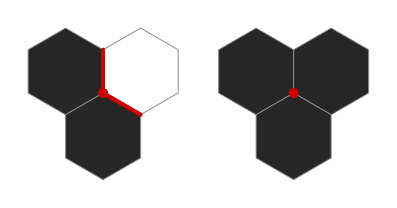
\begin{tikzpicture}[x=0.55cm,y=0.55cm]
    \filldraw[stoneblack] (0.866,-0.500)--(0,-1.000)--(-0.866,-0.500)--(-0.866,0.500)--(0,1.000)--(0.866,0.500)--cycle;
\filldraw[stonewhite] (2.598,-0.500)--(1.732,-1.000)--(0.866,-0.500)--(0.866,0.500)--(1.732,1.000)--(2.598,0.500)--cycle;
\filldraw[stoneblack] (1.732,-2.000)--(0.866,-2.500)--(0,-2.000)--(0,-1.000)--(0.866,-0.500)--(1.732,-1.000)--cycle;
\draw[walk] (0.866,-0.500)--(0.866,0.500);
\draw[walk] (1.732,-1.000)--(0.866,-0.500);
\fill[endpoint] (0.866,-0.500) circle (0.12);
\filldraw[stoneblack] (5.266,-0.500)--(4.400,-1.000)--(3.534,-0.500)--(3.534,0.500)--(4.400,1.000)--(5.266,0.500)--cycle;
\filldraw[stoneblack] (6.998,-0.500)--(6.132,-1.000)--(5.266,-0.500)--(5.266,0.500)--(6.132,1.000)--(6.998,0.500)--cycle;
\filldraw[stoneblack] (6.132,-2.000)--(5.266,-2.500)--(4.400,-2.000)--(4.400,-1.000)--(5.266,-0.500)--(6.132,-1.000)--cycle;
\fill[endpoint] (5.266,-0.500) circle (0.12);

  \end{tikzpicture}
  \caption{The two cases at a vertex of the tiling. Left: the colours split two against one and exactly two fences meet at the vertex. Right: all three cells have the same colour and no fence meets it.}\label{fig:vertex}
\end{figure}

\begin{proposition}\label{prop:existence}
Every colouring of $H_n$ has a black crossing or a white crossing.
\end{proposition}

\begin{proof}
Let $s$ be the vertex of degree $1$ at the top-left corner, where the black frame cell $(-1,0)$ meets the white frame cell $(0,-1)$. Start at $s$ and walk along fences, never using the same fence twice. By Lemma~\ref{lem:degrees}, whenever the walk enters a vertex of degree $2$ it can leave by the other fence. It cannot enter a vertex for the second time, since that vertex would need at least three fences, and it cannot return to $s$, which has degree $1$. Since $G$ is finite, the walk stops at a vertex $t \ne s$ of degree $1$, which is one of the other three corners.

Every fence on the walk has a black cell on one side and a white cell on the other. Let $K_B$ and $K_W$ be the sets of black and white cells that border the walk. Two consecutive fences meet at a vertex where the colours split two against one. If the minority cell is black, both fences border the same black cell; if it is white, the two fences border the two black cells at that vertex, which are adjacent. Hence consecutive black cells along the walk are equal or adjacent, so $K_B$ is connected; the same argument shows that $K_W$ is connected. At $s$, $K_B$ contains a cell of the top frame row and $K_W$ contains a cell of the left frame column.

Suppose $t$ is at the bottom-right or bottom-left corner. At $t$ the walk borders a black cell that lies in the bottom frame row or in row $n-1$, so $K_B$ joins the top frame row to row $n-1$ or below. Take a sequence of adjacent cells of $K_B$ that does this, and consider the part of it after its last visit to row $-1$ and up to its first visit to row $n-1$. All these cells are black board cells (the only other black cells are in rows $-1$ and $n$), the first one is in row $0$ and the last one in row $n-1$. This is a black crossing. If $t$ is at the top-right corner, the same argument applied to $K_W$ and columns gives a white crossing.
\end{proof}

\subsection{At most one crossing}

\begin{proposition}[Huneke \cite{huneke}]\label{prop:uniqueness}
No colouring of $H_n$ has both a black crossing and a white crossing.
\end{proposition}

The intuition is that a black chain from top to bottom divides the board into a part to its left and a part to its right, so that a white chain cannot get from one side to the other without passing through a black cell. Making this precise amounts to a discrete version of the Jordan curve theorem. Huneke \cite{huneke} gives a short proof by induction. We do not reproduce it; this is the only result in the paper that we use without proof. Together, Propositions~\ref{prop:existence} and~\ref{prop:uniqueness} prove Theorem~\ref{thm:hex}.

\section{From the Hex theorem to Brouwer's theorem}\label{sec:brouwer}

Let $\Q = [0,1]^2$ with the Euclidean norm $|\cdot|$, and write $x = (x_1, x_2)$ and $f = (f_1, f_2)$.

\begin{theorem}[Brouwer]\label{thm:brouwer}
Every continuous map $f \colon \Q \to \Q$ has a fixed point.
\end{theorem}

To relate cells to points of $\Q$, place cell $(r,c)$ of $H_n$ at
\[
  x(r,c) = \left( \frac{c + 1/2}{n},\; 1 - \frac{r + 1/2}{n} \right) \in \Q .
\]
Row $0$ is at the top and column $0$ on the left. The points of adjacent cells differ by $\pm(1/n, 0)$, $\pm(0, 1/n)$ or $\pm(1/n, 1/n)$, so they are at distance at most $\sqrt{2}/n$. The points of column $n-1$ have $x_1 = 1 - 1/(2n)$ and those of column $0$ have $x_1 = 1/(2n)$; similarly for rows and $x_2$.

\begin{lemma}\label{lem:approx}
Let $f \colon \Q \to \Q$ be continuous and $\eps > 0$. There is a point $x \in \Q$ with $|f_1(x) - x_1| < \eps$ and $|f_2(x) - x_2| < \eps$.
\end{lemma}

\begin{proof}
Since $\Q$ is compact, $f$ is uniformly continuous, so there is $\delta > 0$ such that $|f(x) - f(y)| < \eps$ whenever $|x - y| < \delta$. We may assume $\delta \le \eps$. Choose $n$ with $\sqrt{2}/n < \delta$ and colour the cells of $H_n$, writing $x$ for the point of a cell, by the rule
\begin{itemize}
  \item white if $|f_1(x) - x_1| \ge \eps$;
  \item otherwise black if $|f_2(x) - x_2| \ge \eps$;
  \item otherwise the cell is left uncoloured.
\end{itemize}
Note that White, who connects left to right, receives the cells that $f$ moves far in the horizontal direction.

\emph{There is no white crossing.} Divide the white cells into \emph{east} cells, with $f_1(x) - x_1 \ge \eps$, and \emph{west} cells, with $x_1 - f_1(x) \ge \eps$. Suppose an east cell with point $x$ is adjacent to a west cell with point $y$. Then $|x - y| < \delta$, so $|f(x) - f(y)| < \eps$, and $x_1 - y_1 > -\delta \ge -\eps$. Adding this inequality to $f_1(x) - x_1 \ge \eps$ and $y_1 - f_1(y) \ge \eps$ gives
\[
  f_1(x) - f_1(y) > \eps ,
\]
which contradicts $|f(x) - f(y)| < \eps$. So no east cell is adjacent to a west cell, and every white crossing consists either of east cells only or of west cells only. A cell in column $n-1$ cannot be an east cell, because $f_1(x) \le 1$ gives $f_1(x) - x_1 \le 1/(2n) < \delta \le \eps$. In the same way a cell in column $0$ cannot be a west cell. A white crossing contains a cell of column $0$ and a cell of column $n-1$, so it can be neither all east nor all west. Hence there is no white crossing.

\emph{There is no black crossing.} The black cells satisfy $|f_2(x) - x_2| \ge \eps$, and the same argument with the second coordinate and the rows in place of the columns applies.

If every cell were coloured, Theorem~\ref{thm:hex} would give a black or a white crossing. So at least one cell is uncoloured, and its point $x$ satisfies $|f_1(x) - x_1| < \eps$ and $|f_2(x) - x_2| < \eps$.
\end{proof}

\begin{proof}[Proof of Theorem~\ref{thm:brouwer}]
By Lemma~\ref{lem:approx} there are points $x^{(k)} \in \Q$ with $|f(x^{(k)}) - x^{(k)}| < \sqrt{2}/k$ for $k = 1, 2, \dots$. Since $\Q$ is compact, a subsequence converges to some $x^* \in \Q$. The function $x \mapsto |f(x) - x|$ is continuous, so $|f(x^*) - x^*| = 0$.
\end{proof}

\begin{remark}
The assignment of directions to players is necessary. If the cells with large horizontal displacement were given to Black instead, the argument would not apply, because a black chain from top to bottom does not have to meet the first or last column. For the map \texttt{fold} of Section~\ref{sec:numerics}, this alternative colouring does contain a black crossing for every board size and every $\eps$ we tested.
\end{remark}

\begin{remark}
Gale \cite{gale} also proves the converse implication, so that the two theorems are equivalent, and extends both to $d$ dimensions using a $d$-player version of Hex. The idea of locating an approximate fixed point by following a path also appears in Sperner's lemma and in the algorithms of Scarf \cite{scarf} for computing fixed points.
\end{remark}

\begin{figure}[t]
  \centering
  \begin{subfigure}[b]{0.32\textwidth}
    \centering
    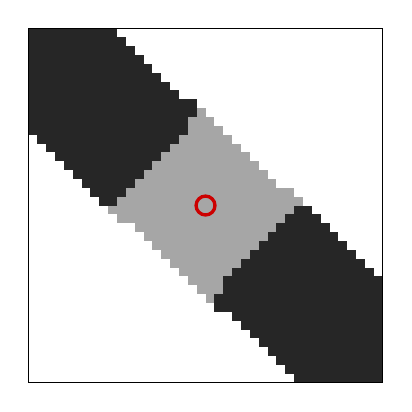
\begin{tikzpicture}[x=0.75cm,y=0.75cm]\fill[gblack] (0,5.850) rectangle (1.500,6.000);
\fill[gwhite] (1.500,5.850) rectangle (6.000,6.000);
\fill[gblack] (0,5.700) rectangle (1.650,5.850);
\fill[gwhite] (1.650,5.700) rectangle (6.000,5.850);
\fill[gblack] (0,5.550) rectangle (1.800,5.700);
\fill[gwhite] (1.800,5.550) rectangle (6.000,5.700);
\fill[gblack] (0,5.400) rectangle (1.950,5.550);
\fill[gwhite] (1.950,5.400) rectangle (6.000,5.550);
\fill[gblack] (0,5.250) rectangle (2.100,5.400);
\fill[gwhite] (2.100,5.250) rectangle (6.000,5.400);
\fill[gblack] (0,5.100) rectangle (2.250,5.250);
\fill[gwhite] (2.250,5.100) rectangle (6.000,5.250);
\fill[gblack] (0,4.950) rectangle (2.400,5.100);
\fill[gwhite] (2.400,4.950) rectangle (6.000,5.100);
\fill[gblack] (0,4.800) rectangle (2.550,4.950);
\fill[gwhite] (2.550,4.800) rectangle (6.000,4.950);
\fill[gblack] (0,4.650) rectangle (2.850,4.800);
\fill[gwhite] (2.850,4.650) rectangle (6.000,4.800);
\fill[gblack] (0,4.500) rectangle (2.850,4.650);
\fill[gblank] (2.850,4.500) rectangle (3.000,4.650);
\fill[gwhite] (3.000,4.500) rectangle (6.000,4.650);
\fill[gblack] (0,4.350) rectangle (2.700,4.500);
\fill[gblank] (2.700,4.350) rectangle (3.150,4.500);
\fill[gwhite] (3.150,4.350) rectangle (6.000,4.500);
\fill[gblack] (0,4.200) rectangle (2.700,4.350);
\fill[gblank] (2.700,4.200) rectangle (3.300,4.350);
\fill[gwhite] (3.300,4.200) rectangle (6.000,4.350);
\fill[gwhite] (0,4.050) rectangle (0.150,4.200);
\fill[gblack] (0.150,4.050) rectangle (2.550,4.200);
\fill[gblank] (2.550,4.050) rectangle (3.450,4.200);
\fill[gwhite] (3.450,4.050) rectangle (6.000,4.200);
\fill[gwhite] (0,3.900) rectangle (0.300,4.050);
\fill[gblack] (0.300,3.900) rectangle (2.400,4.050);
\fill[gblank] (2.400,3.900) rectangle (3.600,4.050);
\fill[gwhite] (3.600,3.900) rectangle (6.000,4.050);
\fill[gwhite] (0,3.750) rectangle (0.450,3.900);
\fill[gblack] (0.450,3.750) rectangle (2.250,3.900);
\fill[gblank] (2.250,3.750) rectangle (3.750,3.900);
\fill[gwhite] (3.750,3.750) rectangle (6.000,3.900);
\fill[gwhite] (0,3.600) rectangle (0.600,3.750);
\fill[gblack] (0.600,3.600) rectangle (2.100,3.750);
\fill[gblank] (2.100,3.600) rectangle (3.900,3.750);
\fill[gwhite] (3.900,3.600) rectangle (6.000,3.750);
\fill[gwhite] (0,3.450) rectangle (0.750,3.600);
\fill[gblack] (0.750,3.450) rectangle (1.950,3.600);
\fill[gblank] (1.950,3.450) rectangle (4.050,3.600);
\fill[gwhite] (4.050,3.450) rectangle (6.000,3.600);
\fill[gwhite] (0,3.300) rectangle (0.900,3.450);
\fill[gblack] (0.900,3.300) rectangle (1.800,3.450);
\fill[gblank] (1.800,3.300) rectangle (4.200,3.450);
\fill[gwhite] (4.200,3.300) rectangle (6.000,3.450);
\fill[gwhite] (0,3.150) rectangle (1.050,3.300);
\fill[gblack] (1.050,3.150) rectangle (1.650,3.300);
\fill[gblank] (1.650,3.150) rectangle (4.500,3.300);
\fill[gwhite] (4.500,3.150) rectangle (6.000,3.300);
\fill[gwhite] (0,3.000) rectangle (1.200,3.150);
\fill[gblack] (1.200,3.000) rectangle (1.500,3.150);
\fill[gblank] (1.500,3.000) rectangle (4.650,3.150);
\fill[gwhite] (4.650,3.000) rectangle (6.000,3.150);
\fill[gwhite] (0,2.850) rectangle (1.350,3.000);
\fill[gblank] (1.350,2.850) rectangle (4.500,3.000);
\fill[gblack] (4.500,2.850) rectangle (4.800,3.000);
\fill[gwhite] (4.800,2.850) rectangle (6.000,3.000);
\fill[gwhite] (0,2.700) rectangle (1.500,2.850);
\fill[gblank] (1.500,2.700) rectangle (4.350,2.850);
\fill[gblack] (4.350,2.700) rectangle (4.950,2.850);
\fill[gwhite] (4.950,2.700) rectangle (6.000,2.850);
\fill[gwhite] (0,2.550) rectangle (1.800,2.700);
\fill[gblank] (1.800,2.550) rectangle (4.200,2.700);
\fill[gblack] (4.200,2.550) rectangle (5.100,2.700);
\fill[gwhite] (5.100,2.550) rectangle (6.000,2.700);
\fill[gwhite] (0,2.400) rectangle (1.950,2.550);
\fill[gblank] (1.950,2.400) rectangle (4.050,2.550);
\fill[gblack] (4.050,2.400) rectangle (5.250,2.550);
\fill[gwhite] (5.250,2.400) rectangle (6.000,2.550);
\fill[gwhite] (0,2.250) rectangle (2.100,2.400);
\fill[gblank] (2.100,2.250) rectangle (3.900,2.400);
\fill[gblack] (3.900,2.250) rectangle (5.400,2.400);
\fill[gwhite] (5.400,2.250) rectangle (6.000,2.400);
\fill[gwhite] (0,2.100) rectangle (2.250,2.250);
\fill[gblank] (2.250,2.100) rectangle (3.750,2.250);
\fill[gblack] (3.750,2.100) rectangle (5.550,2.250);
\fill[gwhite] (5.550,2.100) rectangle (6.000,2.250);
\fill[gwhite] (0,1.950) rectangle (2.400,2.100);
\fill[gblank] (2.400,1.950) rectangle (3.600,2.100);
\fill[gblack] (3.600,1.950) rectangle (5.700,2.100);
\fill[gwhite] (5.700,1.950) rectangle (6.000,2.100);
\fill[gwhite] (0,1.800) rectangle (2.550,1.950);
\fill[gblank] (2.550,1.800) rectangle (3.450,1.950);
\fill[gblack] (3.450,1.800) rectangle (5.850,1.950);
\fill[gwhite] (5.850,1.800) rectangle (6.000,1.950);
\fill[gwhite] (0,1.650) rectangle (2.700,1.800);
\fill[gblank] (2.700,1.650) rectangle (3.300,1.800);
\fill[gblack] (3.300,1.650) rectangle (6.000,1.800);
\fill[gwhite] (0,1.500) rectangle (2.850,1.650);
\fill[gblank] (2.850,1.500) rectangle (3.300,1.650);
\fill[gblack] (3.300,1.500) rectangle (6.000,1.650);
\fill[gwhite] (0,1.350) rectangle (3.000,1.500);
\fill[gblank] (3.000,1.350) rectangle (3.150,1.500);
\fill[gblack] (3.150,1.350) rectangle (6.000,1.500);
\fill[gwhite] (0,1.200) rectangle (3.150,1.350);
\fill[gblack] (3.150,1.200) rectangle (6.000,1.350);
\fill[gwhite] (0,1.050) rectangle (3.450,1.200);
\fill[gblack] (3.450,1.050) rectangle (6.000,1.200);
\fill[gwhite] (0,0.900) rectangle (3.600,1.050);
\fill[gblack] (3.600,0.900) rectangle (6.000,1.050);
\fill[gwhite] (0,0.750) rectangle (3.750,0.900);
\fill[gblack] (3.750,0.750) rectangle (6.000,0.900);
\fill[gwhite] (0,0.600) rectangle (3.900,0.750);
\fill[gblack] (3.900,0.600) rectangle (6.000,0.750);
\fill[gwhite] (0,0.450) rectangle (4.050,0.600);
\fill[gblack] (4.050,0.450) rectangle (6.000,0.600);
\fill[gwhite] (0,0.300) rectangle (4.200,0.450);
\fill[gblack] (4.200,0.300) rectangle (6.000,0.450);
\fill[gwhite] (0,0.150) rectangle (4.350,0.300);
\fill[gblack] (4.350,0.150) rectangle (6.000,0.300);
\fill[gwhite] (0,0) rectangle (4.500,0.150);
\fill[gblack] (4.500,0) rectangle (6.000,0.150);
\draw[gframe] (0,0) rectangle (6,6);
\draw[fixed] (3.000,3.000) circle (0.16);
\end{tikzpicture}
    \caption{\texttt{swirl}: 228 uncoloured}
  \end{subfigure}\hfill
  \begin{subfigure}[b]{0.32\textwidth}
    \centering
    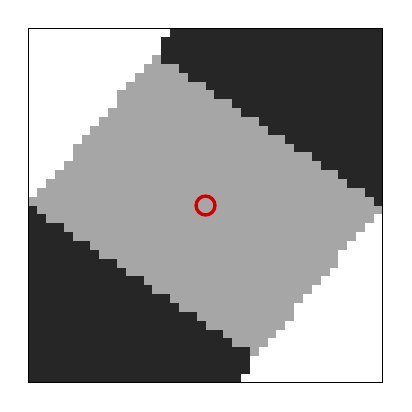
\begin{tikzpicture}[x=0.75cm,y=0.75cm]\fill[gwhite] (0,5.850) rectangle (2.400,6.000);
\fill[gblack] (2.400,5.850) rectangle (6.000,6.000);
\fill[gwhite] (0,5.700) rectangle (2.250,5.850);
\fill[gblack] (2.250,5.700) rectangle (6.000,5.850);
\fill[gwhite] (0,5.550) rectangle (2.250,5.700);
\fill[gblack] (2.250,5.550) rectangle (6.000,5.700);
\fill[gwhite] (0,5.400) rectangle (2.100,5.550);
\fill[gblank] (2.100,5.400) rectangle (2.250,5.550);
\fill[gblack] (2.250,5.400) rectangle (6.000,5.550);
\fill[gwhite] (0,5.250) rectangle (1.950,5.400);
\fill[gblank] (1.950,5.250) rectangle (2.550,5.400);
\fill[gblack] (2.550,5.250) rectangle (6.000,5.400);
\fill[gwhite] (0,5.100) rectangle (1.800,5.250);
\fill[gblank] (1.800,5.100) rectangle (2.700,5.250);
\fill[gblack] (2.700,5.100) rectangle (6.000,5.250);
\fill[gwhite] (0,4.950) rectangle (1.650,5.100);
\fill[gblank] (1.650,4.950) rectangle (3.000,5.100);
\fill[gblack] (3.000,4.950) rectangle (6.000,5.100);
\fill[gwhite] (0,4.800) rectangle (1.500,4.950);
\fill[gblank] (1.500,4.800) rectangle (3.150,4.950);
\fill[gblack] (3.150,4.800) rectangle (6.000,4.950);
\fill[gwhite] (0,4.650) rectangle (1.500,4.800);
\fill[gblank] (1.500,4.650) rectangle (3.450,4.800);
\fill[gblack] (3.450,4.650) rectangle (6.000,4.800);
\fill[gwhite] (0,4.500) rectangle (1.350,4.650);
\fill[gblank] (1.350,4.500) rectangle (3.600,4.650);
\fill[gblack] (3.600,4.500) rectangle (6.000,4.650);
\fill[gwhite] (0,4.350) rectangle (1.200,4.500);
\fill[gblank] (1.200,4.350) rectangle (3.900,4.500);
\fill[gblack] (3.900,4.350) rectangle (6.000,4.500);
\fill[gwhite] (0,4.200) rectangle (1.050,4.350);
\fill[gblank] (1.050,4.200) rectangle (4.050,4.350);
\fill[gblack] (4.050,4.200) rectangle (6.000,4.350);
\fill[gwhite] (0,4.050) rectangle (0.900,4.200);
\fill[gblank] (0.900,4.050) rectangle (4.350,4.200);
\fill[gblack] (4.350,4.050) rectangle (6.000,4.200);
\fill[gwhite] (0,3.900) rectangle (0.750,4.050);
\fill[gblank] (0.750,3.900) rectangle (4.500,4.050);
\fill[gblack] (4.500,3.900) rectangle (6.000,4.050);
\fill[gwhite] (0,3.750) rectangle (0.750,3.900);
\fill[gblank] (0.750,3.750) rectangle (4.800,3.900);
\fill[gblack] (4.800,3.750) rectangle (6.000,3.900);
\fill[gwhite] (0,3.600) rectangle (0.600,3.750);
\fill[gblank] (0.600,3.600) rectangle (4.950,3.750);
\fill[gblack] (4.950,3.600) rectangle (6.000,3.750);
\fill[gwhite] (0,3.450) rectangle (0.450,3.600);
\fill[gblank] (0.450,3.450) rectangle (5.250,3.600);
\fill[gblack] (5.250,3.450) rectangle (6.000,3.600);
\fill[gwhite] (0,3.300) rectangle (0.300,3.450);
\fill[gblank] (0.300,3.300) rectangle (5.400,3.450);
\fill[gblack] (5.400,3.300) rectangle (6.000,3.450);
\fill[gwhite] (0,3.150) rectangle (0.150,3.300);
\fill[gblank] (0.150,3.150) rectangle (5.700,3.300);
\fill[gblack] (5.700,3.150) rectangle (6.000,3.300);
\fill[gblank] (0,3.000) rectangle (5.850,3.150);
\fill[gblack] (5.850,3.000) rectangle (6.000,3.150);
\fill[gblack] (0,2.850) rectangle (0.150,3.000);
\fill[gblank] (0.150,2.850) rectangle (6.000,3.000);
\fill[gblack] (0,2.700) rectangle (0.300,2.850);
\fill[gblank] (0.300,2.700) rectangle (5.850,2.850);
\fill[gwhite] (5.850,2.700) rectangle (6.000,2.850);
\fill[gblack] (0,2.550) rectangle (0.600,2.700);
\fill[gblank] (0.600,2.550) rectangle (5.700,2.700);
\fill[gwhite] (5.700,2.550) rectangle (6.000,2.700);
\fill[gblack] (0,2.400) rectangle (0.750,2.550);
\fill[gblank] (0.750,2.400) rectangle (5.550,2.550);
\fill[gwhite] (5.550,2.400) rectangle (6.000,2.550);
\fill[gblack] (0,2.250) rectangle (1.050,2.400);
\fill[gblank] (1.050,2.250) rectangle (5.400,2.400);
\fill[gwhite] (5.400,2.250) rectangle (6.000,2.400);
\fill[gblack] (0,2.100) rectangle (1.200,2.250);
\fill[gblank] (1.200,2.100) rectangle (5.250,2.250);
\fill[gwhite] (5.250,2.100) rectangle (6.000,2.250);
\fill[gblack] (0,1.950) rectangle (1.500,2.100);
\fill[gblank] (1.500,1.950) rectangle (5.250,2.100);
\fill[gwhite] (5.250,1.950) rectangle (6.000,2.100);
\fill[gblack] (0,1.800) rectangle (1.650,1.950);
\fill[gblank] (1.650,1.800) rectangle (5.100,1.950);
\fill[gwhite] (5.100,1.800) rectangle (6.000,1.950);
\fill[gblack] (0,1.650) rectangle (1.950,1.800);
\fill[gblank] (1.950,1.650) rectangle (4.950,1.800);
\fill[gwhite] (4.950,1.650) rectangle (6.000,1.800);
\fill[gblack] (0,1.500) rectangle (2.100,1.650);
\fill[gblank] (2.100,1.500) rectangle (4.800,1.650);
\fill[gwhite] (4.800,1.500) rectangle (6.000,1.650);
\fill[gblack] (0,1.350) rectangle (2.400,1.500);
\fill[gblank] (2.400,1.350) rectangle (4.650,1.500);
\fill[gwhite] (4.650,1.350) rectangle (6.000,1.500);
\fill[gblack] (0,1.200) rectangle (2.550,1.350);
\fill[gblank] (2.550,1.200) rectangle (4.500,1.350);
\fill[gwhite] (4.500,1.200) rectangle (6.000,1.350);
\fill[gblack] (0,1.050) rectangle (2.850,1.200);
\fill[gblank] (2.850,1.050) rectangle (4.500,1.200);
\fill[gwhite] (4.500,1.050) rectangle (6.000,1.200);
\fill[gblack] (0,0.900) rectangle (3.000,1.050);
\fill[gblank] (3.000,0.900) rectangle (4.350,1.050);
\fill[gwhite] (4.350,0.900) rectangle (6.000,1.050);
\fill[gblack] (0,0.750) rectangle (3.300,0.900);
\fill[gblank] (3.300,0.750) rectangle (4.200,0.900);
\fill[gwhite] (4.200,0.750) rectangle (6.000,0.900);
\fill[gblack] (0,0.600) rectangle (3.450,0.750);
\fill[gblank] (3.450,0.600) rectangle (4.050,0.750);
\fill[gwhite] (4.050,0.600) rectangle (6.000,0.750);
\fill[gblack] (0,0.450) rectangle (3.750,0.600);
\fill[gblank] (3.750,0.450) rectangle (3.900,0.600);
\fill[gwhite] (3.900,0.450) rectangle (6.000,0.600);
\fill[gblack] (0,0.300) rectangle (3.750,0.450);
\fill[gwhite] (3.750,0.300) rectangle (6.000,0.450);
\fill[gblack] (0,0.150) rectangle (3.750,0.300);
\fill[gwhite] (3.750,0.150) rectangle (6.000,0.300);
\fill[gblack] (0,0) rectangle (3.600,0.150);
\fill[gwhite] (3.600,0) rectangle (6.000,0.150);
\draw[gframe] (0,0) rectangle (6,6);
\draw[fixed] (3.000,3.000) circle (0.16);
\end{tikzpicture}
    \caption{\texttt{shear}: 686 uncoloured}
  \end{subfigure}\hfill
  \begin{subfigure}[b]{0.32\textwidth}
    \centering
    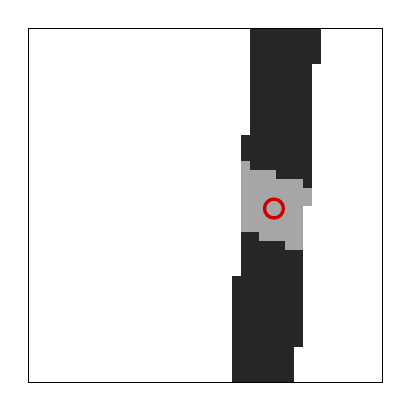
\begin{tikzpicture}[x=0.75cm,y=0.75cm]\fill[gwhite] (0,5.850) rectangle (3.750,6.000);
\fill[gblack] (3.750,5.850) rectangle (4.950,6.000);
\fill[gwhite] (4.950,5.850) rectangle (6.000,6.000);
\fill[gwhite] (0,5.700) rectangle (3.750,5.850);
\fill[gblack] (3.750,5.700) rectangle (4.950,5.850);
\fill[gwhite] (4.950,5.700) rectangle (6.000,5.850);
\fill[gwhite] (0,5.550) rectangle (3.750,5.700);
\fill[gblack] (3.750,5.550) rectangle (4.950,5.700);
\fill[gwhite] (4.950,5.550) rectangle (6.000,5.700);
\fill[gwhite] (0,5.400) rectangle (3.750,5.550);
\fill[gblack] (3.750,5.400) rectangle (4.950,5.550);
\fill[gwhite] (4.950,5.400) rectangle (6.000,5.550);
\fill[gwhite] (0,5.250) rectangle (3.750,5.400);
\fill[gblack] (3.750,5.250) rectangle (4.800,5.400);
\fill[gwhite] (4.800,5.250) rectangle (6.000,5.400);
\fill[gwhite] (0,5.100) rectangle (3.750,5.250);
\fill[gblack] (3.750,5.100) rectangle (4.800,5.250);
\fill[gwhite] (4.800,5.100) rectangle (6.000,5.250);
\fill[gwhite] (0,4.950) rectangle (3.750,5.100);
\fill[gblack] (3.750,4.950) rectangle (4.800,5.100);
\fill[gwhite] (4.800,4.950) rectangle (6.000,5.100);
\fill[gwhite] (0,4.800) rectangle (3.750,4.950);
\fill[gblack] (3.750,4.800) rectangle (4.800,4.950);
\fill[gwhite] (4.800,4.800) rectangle (6.000,4.950);
\fill[gwhite] (0,4.650) rectangle (3.750,4.800);
\fill[gblack] (3.750,4.650) rectangle (4.800,4.800);
\fill[gwhite] (4.800,4.650) rectangle (6.000,4.800);
\fill[gwhite] (0,4.500) rectangle (3.750,4.650);
\fill[gblack] (3.750,4.500) rectangle (4.800,4.650);
\fill[gwhite] (4.800,4.500) rectangle (6.000,4.650);
\fill[gwhite] (0,4.350) rectangle (3.750,4.500);
\fill[gblack] (3.750,4.350) rectangle (4.800,4.500);
\fill[gwhite] (4.800,4.350) rectangle (6.000,4.500);
\fill[gwhite] (0,4.200) rectangle (3.750,4.350);
\fill[gblack] (3.750,4.200) rectangle (4.800,4.350);
\fill[gwhite] (4.800,4.200) rectangle (6.000,4.350);
\fill[gwhite] (0,4.050) rectangle (3.600,4.200);
\fill[gblack] (3.600,4.050) rectangle (4.800,4.200);
\fill[gwhite] (4.800,4.050) rectangle (6.000,4.200);
\fill[gwhite] (0,3.900) rectangle (3.600,4.050);
\fill[gblack] (3.600,3.900) rectangle (4.800,4.050);
\fill[gwhite] (4.800,3.900) rectangle (6.000,4.050);
\fill[gwhite] (0,3.750) rectangle (3.600,3.900);
\fill[gblack] (3.600,3.750) rectangle (4.800,3.900);
\fill[gwhite] (4.800,3.750) rectangle (6.000,3.900);
\fill[gwhite] (0,3.600) rectangle (3.600,3.750);
\fill[gblank] (3.600,3.600) rectangle (3.750,3.750);
\fill[gblack] (3.750,3.600) rectangle (4.800,3.750);
\fill[gwhite] (4.800,3.600) rectangle (6.000,3.750);
\fill[gwhite] (0,3.450) rectangle (3.600,3.600);
\fill[gblank] (3.600,3.450) rectangle (4.200,3.600);
\fill[gblack] (4.200,3.450) rectangle (4.800,3.600);
\fill[gwhite] (4.800,3.450) rectangle (6.000,3.600);
\fill[gwhite] (0,3.300) rectangle (3.600,3.450);
\fill[gblank] (3.600,3.300) rectangle (4.650,3.450);
\fill[gblack] (4.650,3.300) rectangle (4.800,3.450);
\fill[gwhite] (4.800,3.300) rectangle (6.000,3.450);
\fill[gwhite] (0,3.150) rectangle (3.600,3.300);
\fill[gblank] (3.600,3.150) rectangle (4.800,3.300);
\fill[gwhite] (4.800,3.150) rectangle (6.000,3.300);
\fill[gwhite] (0,3.000) rectangle (3.600,3.150);
\fill[gblank] (3.600,3.000) rectangle (4.800,3.150);
\fill[gwhite] (4.800,3.000) rectangle (6.000,3.150);
\fill[gwhite] (0,2.850) rectangle (3.600,3.000);
\fill[gblank] (3.600,2.850) rectangle (4.650,3.000);
\fill[gwhite] (4.650,2.850) rectangle (6.000,3.000);
\fill[gwhite] (0,2.700) rectangle (3.600,2.850);
\fill[gblank] (3.600,2.700) rectangle (4.650,2.850);
\fill[gwhite] (4.650,2.700) rectangle (6.000,2.850);
\fill[gwhite] (0,2.550) rectangle (3.600,2.700);
\fill[gblank] (3.600,2.550) rectangle (4.650,2.700);
\fill[gwhite] (4.650,2.550) rectangle (6.000,2.700);
\fill[gwhite] (0,2.400) rectangle (3.600,2.550);
\fill[gblack] (3.600,2.400) rectangle (3.900,2.550);
\fill[gblank] (3.900,2.400) rectangle (4.650,2.550);
\fill[gwhite] (4.650,2.400) rectangle (6.000,2.550);
\fill[gwhite] (0,2.250) rectangle (3.600,2.400);
\fill[gblack] (3.600,2.250) rectangle (4.350,2.400);
\fill[gblank] (4.350,2.250) rectangle (4.650,2.400);
\fill[gwhite] (4.650,2.250) rectangle (6.000,2.400);
\fill[gwhite] (0,2.100) rectangle (3.600,2.250);
\fill[gblack] (3.600,2.100) rectangle (4.650,2.250);
\fill[gwhite] (4.650,2.100) rectangle (6.000,2.250);
\fill[gwhite] (0,1.950) rectangle (3.600,2.100);
\fill[gblack] (3.600,1.950) rectangle (4.650,2.100);
\fill[gwhite] (4.650,1.950) rectangle (6.000,2.100);
\fill[gwhite] (0,1.800) rectangle (3.600,1.950);
\fill[gblack] (3.600,1.800) rectangle (4.650,1.950);
\fill[gwhite] (4.650,1.800) rectangle (6.000,1.950);
\fill[gwhite] (0,1.650) rectangle (3.450,1.800);
\fill[gblack] (3.450,1.650) rectangle (4.650,1.800);
\fill[gwhite] (4.650,1.650) rectangle (6.000,1.800);
\fill[gwhite] (0,1.500) rectangle (3.450,1.650);
\fill[gblack] (3.450,1.500) rectangle (4.650,1.650);
\fill[gwhite] (4.650,1.500) rectangle (6.000,1.650);
\fill[gwhite] (0,1.350) rectangle (3.450,1.500);
\fill[gblack] (3.450,1.350) rectangle (4.650,1.500);
\fill[gwhite] (4.650,1.350) rectangle (6.000,1.500);
\fill[gwhite] (0,1.200) rectangle (3.450,1.350);
\fill[gblack] (3.450,1.200) rectangle (4.650,1.350);
\fill[gwhite] (4.650,1.200) rectangle (6.000,1.350);
\fill[gwhite] (0,1.050) rectangle (3.450,1.200);
\fill[gblack] (3.450,1.050) rectangle (4.650,1.200);
\fill[gwhite] (4.650,1.050) rectangle (6.000,1.200);
\fill[gwhite] (0,0.900) rectangle (3.450,1.050);
\fill[gblack] (3.450,0.900) rectangle (4.650,1.050);
\fill[gwhite] (4.650,0.900) rectangle (6.000,1.050);
\fill[gwhite] (0,0.750) rectangle (3.450,0.900);
\fill[gblack] (3.450,0.750) rectangle (4.650,0.900);
\fill[gwhite] (4.650,0.750) rectangle (6.000,0.900);
\fill[gwhite] (0,0.600) rectangle (3.450,0.750);
\fill[gblack] (3.450,0.600) rectangle (4.650,0.750);
\fill[gwhite] (4.650,0.600) rectangle (6.000,0.750);
\fill[gwhite] (0,0.450) rectangle (3.450,0.600);
\fill[gblack] (3.450,0.450) rectangle (4.500,0.600);
\fill[gwhite] (4.500,0.450) rectangle (6.000,0.600);
\fill[gwhite] (0,0.300) rectangle (3.450,0.450);
\fill[gblack] (3.450,0.300) rectangle (4.500,0.450);
\fill[gwhite] (4.500,0.300) rectangle (6.000,0.450);
\fill[gwhite] (0,0.150) rectangle (3.450,0.300);
\fill[gblack] (3.450,0.150) rectangle (4.500,0.300);
\fill[gwhite] (4.500,0.150) rectangle (6.000,0.300);
\fill[gwhite] (0,0) rectangle (3.450,0.150);
\fill[gblack] (3.450,0) rectangle (4.500,0.150);
\fill[gwhite] (4.500,0) rectangle (6.000,0.150);
\draw[gframe] (0,0) rectangle (6,6);
\draw[fixed] (4.159,2.949) circle (0.16);
\end{tikzpicture}
    \caption{\texttt{fold}: 56 uncoloured}
  \end{subfigure}
  \caption{Gale's colouring of $H_{40}$ for three maps with $\eps = 0.15$. Each cell is drawn as a square of side $1/40$ centred at its point in $\Q$: black and white as in the proof of Lemma~\ref{lem:approx}, grey for uncoloured cells. The circle marks a fixed point of $f$ computed numerically. No white region joins the left and right sides and no black region joins the top and bottom.}\label{fig:gale}
\end{figure}

\section{Random colourings}\label{sec:perc}

Colour each cell of $H_n$ black with probability $p \in [0,1]$ and white otherwise, independently of the other cells. This is site percolation on a finite piece of the triangular lattice, whose vertices are the centres of the hexagons. Write $\Prob_p$ for the resulting probability measure and
\[
  \theta_n(p) = \Prob_p(\text{there is a black crossing}).
\]

\begin{theorem}\label{thm:half}
For every $n \ge 1$ and $p \in [0,1]$,
\[
  \theta_n(p) + \theta_n(1-p) = 1 .
\]
In particular $\theta_n(1/2) = 1/2$.
\end{theorem}

\begin{proof}
By Theorem~\ref{thm:hex}, exactly one of the events \emph{black crossing} and \emph{white crossing} occurs for every colouring, so
\begin{equation}\label{eq:sum}
  \Prob_p(\text{black crossing}) + \Prob_p(\text{white crossing}) = 1 .
\end{equation}
Let $\tau(r,c) = (c,r)$ be the transposition of the board. It maps the set of differences $\{\pm(0,1), \pm(1,0), \pm(1,-1)\}$ to itself, so it maps adjacent cells to adjacent cells. It also maps row $0$ to column $0$ and row $n-1$ to column $n-1$. Given a colouring $\kappa$, define $\kappa^*$ by giving the cell $\tau(r,c)$ the colour opposite to $\kappa(r,c)$. A sequence of cells is a black crossing for $\kappa$ if and only if its image under $\tau$ is a white crossing for $\kappa^*$. If $\kappa$ has law $\Prob_p$, then the cells of $\kappa^*$ are black independently with probability $1-p$, so $\kappa^*$ has law $\Prob_{1-p}$. Therefore
\[
  \theta_n(p) = \Prob_{1-p}(\text{white crossing}) = 1 - \theta_n(1-p),
\]
where the last step is \eqref{eq:sum} with $1-p$ in place of $p$.
\end{proof}

\begin{remark}
The board must be square. On an $n \times m$ board with $n \ne m$, the transposition does not map the board to itself, and at $p = 1/2$ the player with the shorter distance to cross has a probability of crossing larger than $1/2$. For example, on a board with $4$ rows and $5$ columns, Black crosses in $636\,351$ of the $2^{20} = 1\,048\,576$ colourings, a fraction of about $0.607$.
\end{remark}

\begin{remark}
As $n \to \infty$, $\theta_n(p)$ tends to $0$ for $p < 1/2$ and to $1$ for $p > 1/2$, because $1/2$ is the critical probability for site percolation on the triangular lattice; see Bollob\'as and Riordan \cite{bollobas-riordan}. At $p = 1/2$, Smirnov \cite{smirnov} proved Cardy's formula for the limit of crossing probabilities of general domains. We mention these results for context only; nothing else in the paper depends on them.
\end{remark}

\section{Numerical checks}\label{sec:numerics}

The board logic is written in JavaScript (\texttt{js/hex.js} in the repository). Crossings are detected with a union--find structure that has four virtual nodes for the four edges of the board. The test suite (\texttt{test/logic.test.js}) checks this against an independent breadth-first search on 2000 random boards with $5 \le n \le 11$. All random boards in this section and in the figures are generated with a seeded generator, so the results can be reproduced with \texttt{scripts/make-figures.js}.

\subsection{Exhaustive enumeration}

For small $n$ we enumerated all $2^{n^2}$ colourings of $H_n$ and counted those with a black crossing and those with no crossing at all. The results are in Table~\ref{tab:enum}. For each $n \le 5$ there is no colouring without a crossing, which checks Proposition~\ref{prop:existence} on these boards, and exactly half of the colourings have a black crossing, which is the case $p = 1/2$ of Theorem~\ref{thm:half}. The enumeration for $n = 5$ took about four and a half minutes on our machine.

\begin{table}[h]
  \centering
  \pgfplotstabletypeset[
    col sep=comma,
    columns={n,total,black,none},
    columns/n/.style={column name=$n$, int detect},
    columns/total/.style={column name={colourings $2^{n^2}$}, int detect, column type=r,
      /pgf/number format/1000 sep={\,}},
    columns/black/.style={column name={with black crossing}, int detect, column type=r,
      /pgf/number format/1000 sep={\,}},
    columns/none/.style={column name={with no crossing}, int detect, column type=r},
    every head row/.style={before row=\toprule, after row=\midrule},
    every last row/.style={after row=\bottomrule},
  ]{data/enumeration.csv}
  \caption{Exhaustive enumeration of all colourings of $H_n$.}\label{tab:enum}
\end{table}

\subsection{Crossing probabilities}

Figure~\ref{fig:theta} shows Monte Carlo estimates of $\theta_n(p)$ for $n = 5, 11, 21, 35$ and $p = 0.30, 0.32, \dots, 0.70$, with $20\,000$ boards for each pair $(n,p)$, so that each estimate has a standard error of at most $0.0036$. The curves pass through $(1/2, 1/2)$ and are symmetric under $(p, \theta) \mapsto (1-p, 1-\theta)$, as Theorem~\ref{thm:half} requires. They become steeper as $n$ grows, which is consistent with the critical behaviour described in the last remark of Section~\ref{sec:perc}.
\pgfplotstableread[col sep=comma]{data/crossing.csv}\crossingtable
\pgfplotstablegetelem{5}{theta5}\of\crossingtable\let\thetaA\pgfplotsretval
\pgfplotstablegetelem{5}{theta35}\of\crossingtable\let\thetaB\pgfplotsretval
\pgfplotstablegetelem{10}{theta35}\of\crossingtable\let\thetaC\pgfplotsretval
For example, at $p = 0.40$ the estimate is $\thetaA$ for $n = 5$ and $\thetaB$ for $n = 35$, and at $p = 1/2$ the estimate for $n = 35$ is $\thetaC$.

\begin{figure}[t]
  \centering
  \begin{tikzpicture}
    \begin{axis}[
      width=0.78\textwidth, height=0.5\textwidth,
      xlabel={$p$}, ylabel={$\theta_n(p)$},
      xmin=0.29, xmax=0.71, ymin=-0.02, ymax=1.02,
      xtick={0.3,0.4,0.5,0.6,0.7}, ytick={0,0.25,0.5,0.75,1},
      grid=major, grid style={black!12},
      legend pos=north west, legend cell align=left,
      tick label style={font=\small}, label style={font=\small}, legend style={font=\small},
      every axis plot/.append style={line width=0.9pt},
    ]
      \addplot[black!30, mark=*, mark size=1.2pt] table[x=p, y=theta5, col sep=comma] {data/crossing.csv};
      \addplot[black!55, mark=square*, mark size=1.2pt] table[x=p, y=theta11, col sep=comma] {data/crossing.csv};
      \addplot[black!75, mark=triangle*, mark size=1.5pt] table[x=p, y=theta21, col sep=comma] {data/crossing.csv};
      \addplot[red!80!black, mark=diamond*, mark size=1.5pt] table[x=p, y=theta35, col sep=comma] {data/crossing.csv};
      \legend{$n=5$, $n=11$, $n=21$, $n=35$}
    \end{axis}
  \end{tikzpicture}
  \caption{Monte Carlo estimates of the probability $\theta_n(p)$ of a black crossing on $H_n$; $20\,000$ boards per point.}\label{fig:theta}
\end{figure}

\subsection{Gale's colouring}

The test suite also checks Lemma~\ref{lem:approx} on three continuous maps of $\Q$ into itself, defined in \texttt{js/maps.js}: a rotation about the centre combined with a contraction (\texttt{swirl}), an affine map (\texttt{shear}), and a map involving $|x_1 - 0.35|$ and $\sin(5x_1)$ (\texttt{fold}). For each map, each $n \in \{40, 60, 80\}$ and each $\eps \in \{0.15, 0.25, 0.4\}$, the test colours $H_n$ by the rule in the proof of Lemma~\ref{lem:approx}. It first checks the hypotheses that the proof uses: $|f(x) - f(y)| < \eps$ for the points $x, y$ of every pair of adjacent cells, and $1/n < \eps$. It then checks with the same crossing detection as above that neither player has a crossing, that at least one cell is uncoloured, and that every uncoloured cell satisfies $|f(x) - x| < \sqrt{2}\,\eps$. All 27 cases pass. Figure~\ref{fig:gale} shows the colourings for $n = 40$ and $\eps = 0.15$.


\subsection{Interactive version}

The repository also contains a web page with four interactive versions of the material above: a two-player Hex board, a step-by-step version of the walk in Figure~\ref{fig:walk} on random boards, Gale's colouring for a chosen map, mesh and $\eps$, and a Monte Carlo simulator for $\theta_n(p)$.

\section*{Acknowledgments}

Claude (Anthropic) was used to assist with refining and reviewing the mathematical exposition, verifying results, and debugging code. The authors retain full responsibility for the final content and its correctness.

\begin{thebibliography}{9}

\bibitem{bollobas-riordan}
B.~Bollob\'as and O.~Riordan, \emph{Percolation}, Cambridge University Press, 2006.

\bibitem{gale}
D.~Gale, The game of Hex and the Brouwer fixed-point theorem, \emph{Amer. Math. Monthly} \textbf{86} (1979), no.~10, 818--827. \href{https://doi.org/10.2307/2320146}{doi:10.2307/2320146}.

\bibitem{gardner}
M.~Gardner, Mathematical games: Concerning the game of Hex, which may be played on the tiles of the bathroom floor, \emph{Scientific American} \textbf{197} (July 1957). Reprinted in \emph{The Scientific American Book of Mathematical Puzzles and Diversions}, Simon \& Schuster, 1959.

\bibitem{hayward-toft}
R.~B.~Hayward and B.~Toft, \emph{Hex: The Full Story}, CRC Press, 2019.

\bibitem{huneke}
C.~Huneke, An inductive proof of Hex uniqueness, \emph{Amer. Math. Monthly} \textbf{121} (2014), no.~1, 78--80. \href{https://doi.org/10.4169/amer.math.monthly.121.01.078}{doi:10.4169/amer.math.monthly.121.01.078}.

\bibitem{scarf}
H.~Scarf, The approximation of fixed points of a continuous mapping, \emph{SIAM J. Appl. Math.} \textbf{15} (1967), no.~5, 1328--1343.

\bibitem{smirnov}
S.~Smirnov, Critical percolation in the plane: conformal invariance, Cardy's formula, scaling limits, \emph{C. R. Acad. Sci. Paris S\'er. I Math.} \textbf{333} (2001), no.~3, 239--244.

\end{thebibliography}

\end{document}
